\documentclass{article}
\usepackage[T1]{fontenc}
\usepackage{lmodern}
\usepackage{graphicx}
\usepackage{amsmath,amssymb}
\usepackage[a4paper,margin=2cm]{geometry}
\usepackage[absolute,overlay]{textpos}
\setlength{\TPHorizModule}{1mm}
\setlength{\TPVertModule}{1mm}
\usepackage[indonesian]{babel}
\usepackage{hyperref}
\setlength{\emergencystretch}{2em}
% unit: Halaman 44

\begin{document}

% === Halaman 44 (llm) ===

\section*{Metode LSB}

\begin{itemize}
    \item Di dalam setiap $byte$ bit-bitnya tersusun dari kiri ke kanan dalam urutan yang kurang berarti (\textit{least significant bits} atau LSB) hingga bit-bit yang berarti (\textit{most significant bits} atau MSB).
    \item Susunan bit pada setiap $byte$ adalah $b_7b_6b_5b_4b_3b_2b_1b_0$.
\end{itemize}

Contoh:

\vspace{30mm}

\begin{align*}
\text{Nilai dalam desimal} &= 1 \times 2^7 + 1 \times 2^6 + 0 \times 2^5 + 1 \times 2^4 + 0 \times 2^3 + 0 \times 2^2 + 0 \times 2^1 + 1 \times 2^0 = 209
\end{align*}

% deskripsi: Ilustrasi penentuan MSB (Most Significant Bit) dan LSB (Least Significant Bit) pada sebuah deret biner 11010001 menggunakan panah penunjuk.
% bbox normalisasi: [0.1900, 0.5800, 0.4080, 0.8200]
\begin{textblock*}{45.78mm}(39.90mm,172.26mm)
\noindent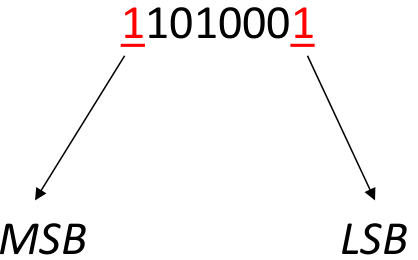
\includegraphics[width=45.78mm,height=71.28mm]{../../images/llm/page_044_img_01.png}%
\end{textblock*}

\end{document}
